\chapter{Nyomtatási beállítások}
\thispagestyle{empty}

A munkalap nyomtatása előtt a Standard eszköztár vagy a Fájl
menü Nyomtatási kép parancsával megtekinthetjük a
dokumentumunk nyomtatási előnézetét (\ref{NyomtatásiKép} ábra). Az
ablakban ránagyíthatunk a dokumentumra, lapozhatjuk a nyomtatásra
kerülő oldalakat.

\begin{figure}[!h]
\begin{center}
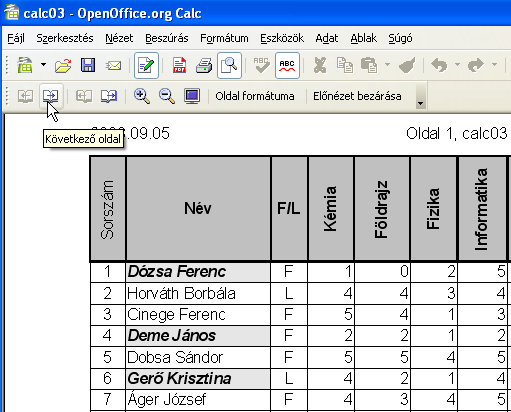
\includegraphics[width=12.52cm]{oocalcv1-img164.png}
\caption{Nyomtatási kép}\label{NyomtatásiKép}
\end{center}
\end{figure}

Az \textbf{Oldal formátuma} kapcsolóval módosíthatjuk a
nyomtatási beállításokat. Amennyiben nem hoztunk létre és
alkalmaztunk másik oldalstílust, az alapértelmezett oldalstílus
beállításait látjuk. Az ablak első \textbf{Szervező} nevű fülén a stílus
rövid tartalmát látjuk. 


\section{Oldalbeállítás}

A második fülre kattintva az oldal beállításait adhatjuk meg
(\ref{Oldalbeállítás} ábra). Itt választhatunk papírformátumot és
\textbf{Tájolás} csoportban beállíthatjuk, hogy a nyomtatás
\textbf{Álló} vagy \textbf{Fekvő} oldalra történjen. A
\textbf{Margók} részben megadhatjuk, hogy a szöveg és a papír
szélei között mekkora szabad hely legyen. A Táblázat
igazításánál megadhatjuk, hogy vízszintesen és
függőlegesen középre rendezze a cellákat a nyomtatott
oldalon.

\begin{figure}[!h]
\begin{center}
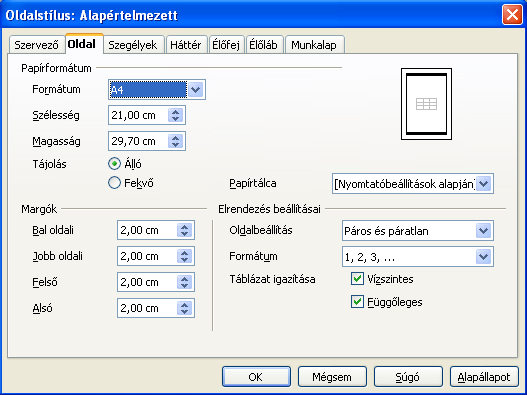
\includegraphics[width=12.944cm]{oocalcv1-img165.png}
\caption{Oldalbeállítás}\label{Oldalbeállítás}
\end{center}
\end{figure}


\section{Élőfej és élőláb}

Az Élőfej és Élőláb fülek segítségével
beállíthatjuk az oldal tetején és alján megjelenő
szöveget. A Szerkesztés kapcsolóval beállíthatjuk, hogy
milyen információ jelenjen meg az oldal közepén illetve bal-
és jobb oldalán (\ref{Élőfej} ábra).

\begin{figure}[!h]
\begin{center}
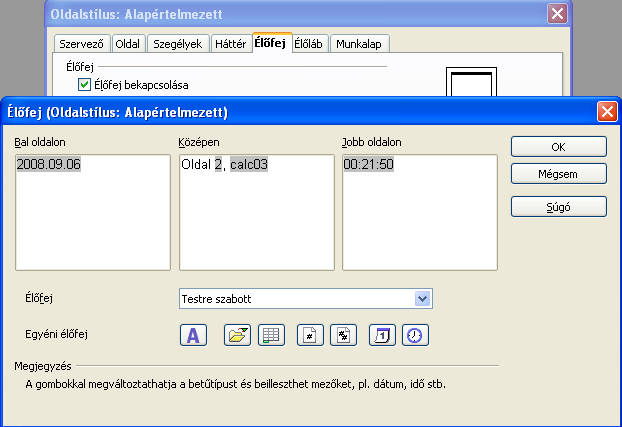
\includegraphics[width=14.999cm]{oocalcv1-img166.png}
\caption{Élőfej}\label{Élőfej}
\end{center}
\end{figure}

Az \textbf{Élőfej} sorban választhatunk az előre
meghatározott tartalmak közül, az \textbf{Egyéni élőfej}
sorában található kapcsolókkal pedig beilleszthetünk
mezőket az egérrel kiválasztott ablakok valamelyikébe.


\section{Munkalap}

Az utolsó, \textbf{Munkalap} fülön beállíthatjuk a
nyomtatási sorrendet, az első oldalszámot, illetve az oldal
méretezését is. Megadhatjuk, hogy a munkalap tartalmán
kívül a \textbf{Sor- és oszlopfejlécek} és a \textbf{Rács}
is nyomtatásra kerüljön. A \textbf{Képletek} kapcsoló
bekapcsolásával a számított cellák képletit nyomtatja ki,
nem pedig azok eredményeit.

Három méretezésmódot választhatunk (\ref{Munkalap} ábra). Az
elsőnél megadhatjuk a méretezés faktorát
százalékértékkel. A másodikat választva meghatározhatjuk,
hogy a kinyomtatott munkalap hány oldalnyi legyen magasságban és
szélességben. A harmadik lehetőséggel az oldalak számát
adhatjuk meg, és a Calc úgy csökkenti méretarányt, hogy a
tartalom ráférjen a megadott oldalszámra.

\begin{figure}[!h]
\begin{center}
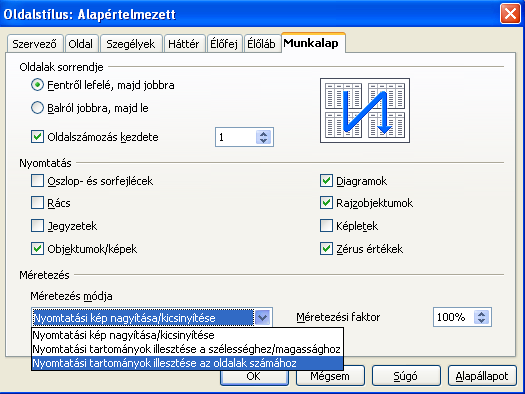
\includegraphics[width=12.891cm]{oocalcv1-img167.png}
\caption{Munkalap}\label{Munkalap}
\end{center}
\end{figure}


\section{Nyomtatási tartomány meghatározása}

A Calcban meghatározhatunk a munkalapon egy tartományt nyomtatási
területként, ha nem szükséges a teljes munkalapot kinyomtatni.
Legegyszerűbben ezt a tartományt kijelölve a
\textbf{Formátum} menüpont \textbf{Nyomtatandó tartomány}
\textbf{Meghatározás} paranccsal tehetjük meg. Több
tartományt is meghatározhatunk, ugyanitt a \textbf{Hozzáadás}
parancs segítségével. Az \textbf{Eltávolítás} parancs
megszünteti a megadott nyomtatási területet. A
\textbf{Szerkesztés} segítségével megnyithatunk egy
párbeszédablakot, amelyen látjuk az eddig meghatározott
tartományokat és módosíthatjuk is azokat (\ref{NyomtatásiTartomány} ábra).

\begin{figure}[!h]
\begin{center}
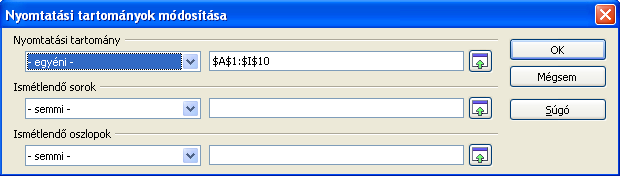
\includegraphics[width=14.999cm]{oocalcv1-img168.png}
\caption{Nyomtatási tartomány megadása}\label{NyomtatásiTartomány}
\end{center}
\end{figure}


\section{Ismétlődő sorok és oszlopok}

Több oldalas táblázatok nyomtatásánál hasznos lehet, ha egy
sor vagy oszlop minden kinyomtatott oldalon megjelenik. A
\textbf{Nyomtatási tartományok módosítása} párbeszédablak
megfelelő soraiban  meghatározhatunk ilyen sorokat vagy
oszlopokat.

Az első oszlop és sor minden oldalra kinyomtatásához az A1
cellára kell kattintani mind az ismétlődő sorok, mind az
ismétlődő oszlopok résznél. Ezt a beállítást az itt
megjelenő \$1 és \$A kifejezések jelzik.


\section{Nyomtatás}

Az \textbf{Standard} eszköztár \textbf{Fájl közvetlen
nyomtatása} parancsával az aktív munkalap vagy a kijelölt
munkalapok nyomtatását indítja a program az alapértelmezett
beállításokkal. A Fájl menü Nyomtatás parancsával
megjelenő párbeszédablakban módosíthatók az aktuális
dokumentum nyomtatási beállításai (\ref{Nyomtatás} ábra). Több
telepített nyomtató esetén kiválaszthatjuk, hogy melyikre
történjen a nyomtatás. Megadhatjuk, hogy a \textbf{Kijelölt
munkalapok}, \textbf{Minden munkalap}, vagy csak a \textbf{Kijelölt
cellák} kerüljenek nyomtatásra. Megadhatjuk, hogy mely oldalakat
nyomtassa ki a program. Összefüggő oldaltartomány
nyomtatásához használhatjuk a 3--6 formátumot. Különálló
oldalak nyomtatásánál az oldalszámok közé írjunk
pontosvesszőt.

\begin{figure}[!h]
\begin{center}
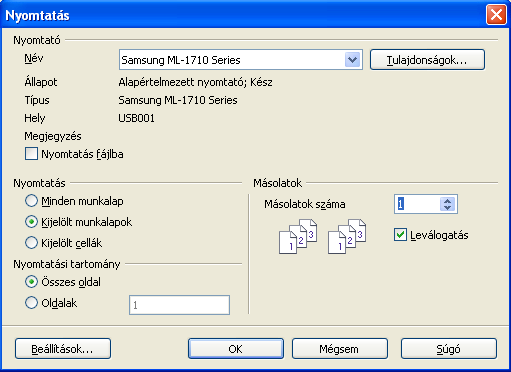
\includegraphics[width=12.52cm]{oocalcv1-img169.png}
\caption{Nyomtatás}\label{Nyomtatás}
\end{center}
\end{figure}

